% REV00 Tue 20 Jul 2021 08:12:01 WIB
% START Tue 20 Jul 2021 08:12:01 WIB

\chapter{Kedua}

% 11
\begin{figure}[htbp]
% h: here, where the figure appears in the text (use can always just use [h] )
% t: top,  top of the current page.
% b: bottom of the current page.
% p: page, top of the next available float space (sometimes end up being the end of the document).
\centerline{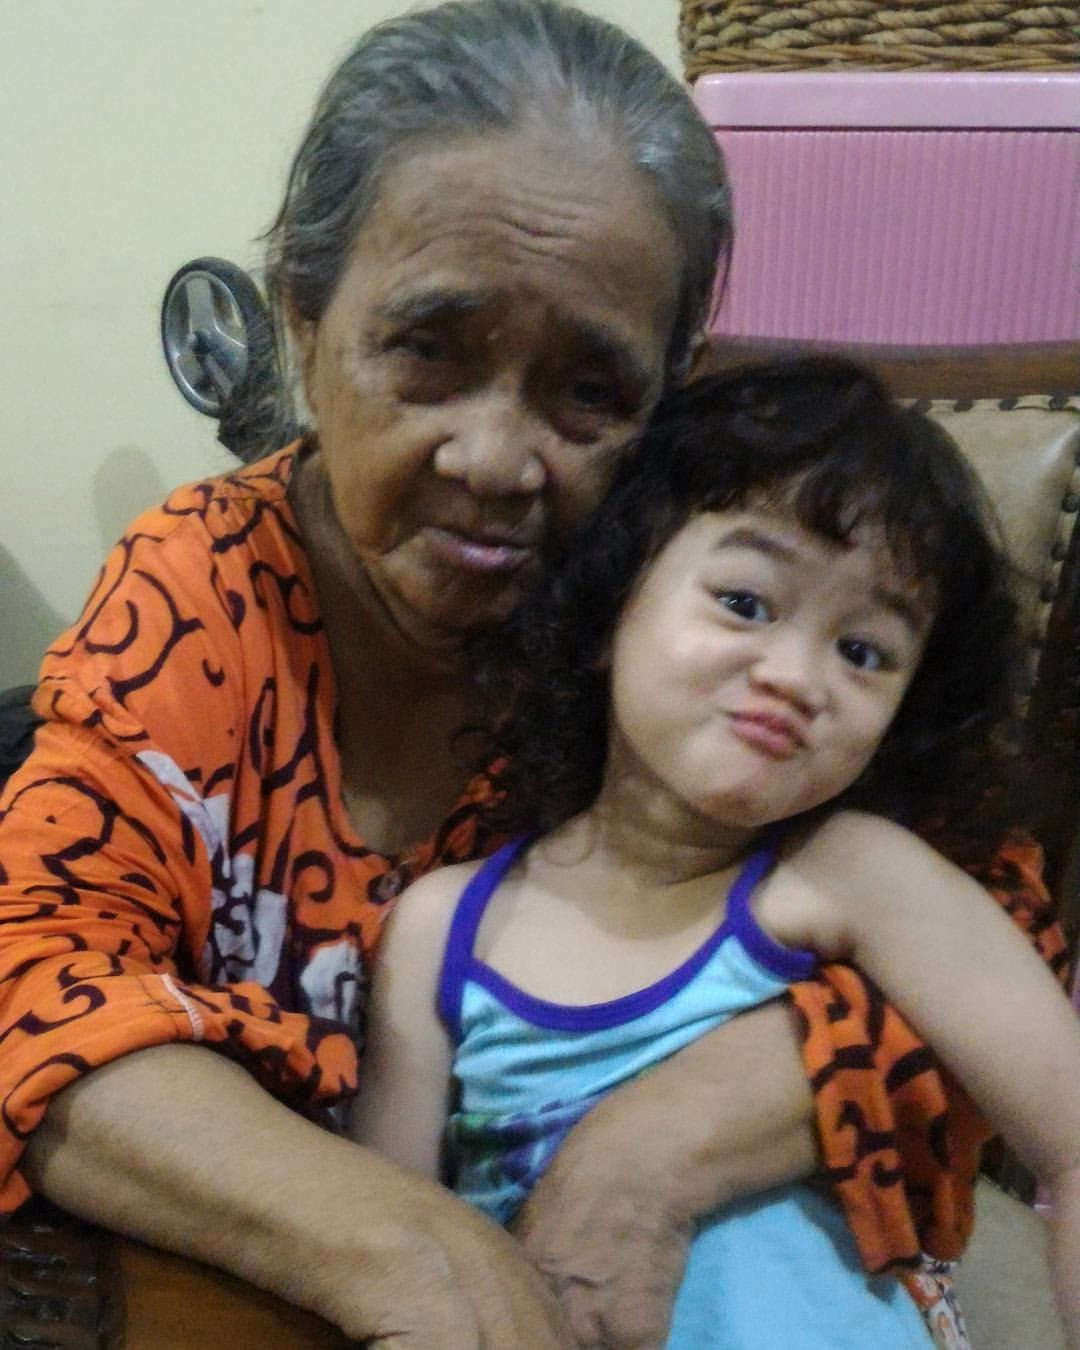
\includegraphics[scale=1.1]{01-02-01}}
\caption{Ibuda tersayang Bang Tiri, yang biasanya dipanggil "iie". Al Fatihah buat ibunda iie.}
\label{01-02-01}
\end{figure}
%

Kalaupun Satiri kecil tersaruk-saruk, beranjak remaja dengan segudang tantangan, dan kemudian 'terdampar' di kampus Ganesha, dia tidak pernah berhenti bersenang-senang bersama-teman-teman. Dia bukan tipe serius penyendiri. Dan kampus ITB itu pun ternyata baginya hanya sebatas persinggahan. Perjalanannya masih jauh ke dapan.

Tahun 1967, di jaman yang sulit itu, saya masuk Sekolah Dasar (SD). Satiri setahun lebih tua dari saya. Sebagai orang pendatang, saya tahu bahwa saat itu masyarakat Betawi di tempat kami banyak yang tidak bersekolah. Kalaupun ada yang bersekolah, nyaris tidak ada yang kuliah.

Bagaimana dengan Satiri? Ya sama saja dengan yang lainnya, main di tegalan sawah, berceloteh di ladang, bergembira sepanjang hari. Hingga suatu hari, Tuhan menurunkan guru pertama baginya. Katakanlah namanya Saifullah. (Tentu saja saya tidak tahu nama sebenarnya). Bang Ipul, katakanlah begitu panggilan akrabnya karena dia juga orang Betawi asli, adalah lulusan Sekolah Pendidikan Guru (SPG), setingkat SMA. Pada saat itu, lulusan SPG sudah merupakan suatu previlese.

Pagi Bang Ipul mengajar di SD Palmerah. Siang yang berkepanjangan di rumahnya, ia tidak mungkin untuk menjadi suntuk dengan ramainya canda ria, banyolan-banyolan anak-anak yang saling ejek khas betawi. Anak-anak itu tidak ada yang bersekolah. Karena iseng, Bang Ipul seraya meneriaki mereka:

"Eh Tong, elu pade mao maen sekola-sekolaan kagak?" (Hi kids, do you all wanna play like in school?)

"Maooo", seru anak-anak serempak bergembira.

Begitulah, meja ping-pong dijadikan papan tulis, dengan bangku kayu pendek (jengkok, dingklik atau jojodog) sebagai kursi yang nyaman bagi enam anak-anak merdeka. Kapur tulis adalah senjata utamanya. Belakangan Bang Ipul membuatkan papan-papan kecil sebagai "buku tulis" bagi anak-anak. Buku bacaan? Hanya Bang Ipul yang punya, dan boleh dibaca sepanjang hari. Mesin foto copy tentu belum ditemukan. Listrik pun belum dikenal di Rawa Belong.

Bang Ipul tentu saja mulai dengan mengajarkan anak-anak mengenal huruf dan angka. Ini Satiri kecil bawel luar biasa, bertanya terus dia. Bicara tidak ada capeknya. Bang Ipul kewalahan, tetapi senang bukan kepalang. Setelah bisa membaca, Satiri segera membacai buku-buku yang ada di rumah Bang Ipul. Begitupun tetap saja tidak mau kalah dalam main petak umpet, main gasing, gatrik, kelereng ataupun kejar layangan.

"Bang Ipul, minyak itu asalnya dari mana si, koq bisa nyala kalau dibakar?"

"Itu dari perut bumi bla, bla, bla"

"Kalau Radio kenapa bisa bunyi ya, kan enggak ada orangnya?"

"Itu elekronika bla, bla, bla"

"Elektronika?"

Bang Ipul segera tahu perbedaan Satiri, sehingga tak lama berselang meja ping-pong dibagi dua. Sebelah kanan khusus buat Satiri, sisanya buat anak-anak yang lain. Begitulah hari-hari berlalu hingga tahun ke-5, 1972.

Tahun itu, baba (ayah) Satiri sakit keras, mungkin semacam tifus. Berminggu-minggu hanya terbaring di rumah. Lalu bagaimana keluarga ini bertahan?

Selepas mencium tangan ibundanya dan memohon doa, Satiri kecil pelan-pelan mengeluarkan sepeda babanya agar tidak menggangu baba yang sedang meriang. Sobat-sobatnya mengingat betul kebiasaan Satiri mencium tangan ibunya dan meminta doa setiap akan bepergian.

Berangkatlah ia ke medan perang. Satiri menaiki sepeda batangan ayahnya dengan satu kaki berada di bawah batangan sepeda itu. Sedapat-dapatnya ia mencari kembang dari kebun-kebun kosong dan semak belukar. Termasuk mawar, kembang sepatu dan kembang kemboja yang diambil dari pohon-pohon di sekitar pemakaman. Kembang-kembang itu dijualnya di pasar Kebayoran Lama dan Blok M. Itu artinya Satiri kecil, berusia sebelas tahun, mengayuh sepeda dengan gaya miring sejauh tak kurang dari 20 km setiap hari. Selama beberapa minggu.

Anda boleh mengatakan bahwa malaikat-malaikat sudah membantunya. Yang sebenarnya juga: Ibunda dan adik-adiknya selalu menunggu kedatangan Satiri dengan penuh harapan. Pandangan mata mereka yang cuma satu-dua detik itulah yang memberinya kekuatan hingga berpuluh-puluh tahun kemudian.

It's definitely a quantum leap. A glimpse of time turns into an immortality.

Tuhan menyembuhkan ayahnya, dan gurunya pun tidak lagi memiliki apapun untuk diajarkan kepadanya sebagai anak SD. Tanpa sepengetahuan ayahnya, Bang Ipul mendaftarkan Satiri untuk diikutkan ujian negara tingkat SD di SD Palmerah. Tidak ada kegemparan ketika diumumkan bahwa nilai Satiri adalah yang tertinggi sekecamatan, mengalahkan nilai semua anak yang setiap hari datang ke sekolah. Siapa pula yang mengenal siswa Satiri selain Bang Ipul?

Ijazah SD itu hanya disimpan di lemari pakaian orang tuanya, satu-satunya barang berharga di rumah. Ijazah mengkilap yang sunyi, kesepian, tanpa arti.

Bagi orang tuanya, dan kebanyakan orang tua Betawi saat itu, pendidikan terpenting bukanlah sekolah. Yang diutamakan adalah mengaji di Langgar (mesjid kecil, surau). Oh, jangan tanya, untuk urusan ngaji pun Satiri tidak mau kalah, bertahun-tahun hingga SMA pun ia juara Tilawah Quran.

Bulan-bulan pun berlalu tanpa sekolah. Dan itu artinya waktu untuk bersenang-senang.

Di sela-sela itu, Tuhan mencatat kata 'minyak' dan 'elektronika' yang ditanyakan Satiri kepada bang Ipul.
\\[10pt]


Sumber tulisan asli \url{https://www.facebook.com/reno.alamsyah.94/posts/10226511661043875}

